%%%%%%%%%%%%%%%%%%%%%%%%%%%%%%%%%%%%%%%%%
% Beamer Presentation
% LaTeX Template
% Version 1.0 (10/11/12)
%
% This template has been downloaded from:
% http://www.LaTeXTemplates.com
%
% License:
% CC BY-NC-SA 3.0 (http://creativecommons.org/licenses/by-nc-sa/3.0/)
%
%%%%%%%%%%%%%%%%%%%%%%%%%%%%%%%%%%%%%%%%%

%----------------------------------------------------------------------------------------
%	PACKAGES AND THEMES
%----------------------------------------------------------------------------------------

\documentclass[14pt]{beamer}

\mode<presentation> {

% The Beamer class slide themes
\usetheme{Madrid} %i was using this one

% Beamer class color themes

%\usecolortheme{albatross}

%\setbeamertemplate{footline} % To remove the footer line in all slides uncomment this line
%\setbeamertemplate{footline}[page number] % To replace the footer line in all slides with a simple slide count uncomment this line

%\setbeamertemplate{navigation symbols}{} % To remove the navigation symbols from the bottom of all slides uncomment this line
}

\usepackage{graphicx} % Allows including images
\usepackage{booktabs} % Allows the use of \toprule, \midrule and \bottomrule in tables
\usepackage{hyperref}
\usepackage{helvet}

%----------------------------------------------------------------------------------------
%	TITLE PAGE
%----------------------------------------------------------------------------------------

\title[Genomics]{Genetics v Genomics} % The short title appears at the bottom of every slide, the full title is only on the title page

\author{C. Ryan Campbell} % Your name
\institute[Duke] % Your institution as it will appear on the bottom of every slide, may be shorthand to save space
{
Duke University \\ % Your institution for the title page
\medskip
\textit{c.ryan.campbell@duke.edu} % Your email address
}
\date{05 Sept 2017} % Date, can be changed to a custom date

\begin{document}

\begin{frame}
\titlepage % Print the title page as the first slide
\end{frame}

\begin{frame}
\frametitle{Overview} % Table of contents slide, comment this block out to remove it
\tableofcontents % Throughout your presentation, if you choose to use \section{} and \subsection{} commands, these will automatically be printed on this slide as an overview of your presentation
\end{frame}

%----------------------------------------------------------------------------------------
%	PRESENTATION SLIDES
%----------------------------------------------------------------------------------------

%------------------------------------------------
\section{Genetics v. Genomics} 
%------------------------------------------------

\subsection{Goals} 

%------------------------------------------------
\begin{frame}
\frametitle{Today's Goals}
%what students should know/learn today
\begin{itemize}
	\item What is/are Genomics?
	\item How have techniques changed?
	\item What impact has that had on biological questions?
	%\sffamily
\end{itemize}
\end{frame}


%------------------------------------------------
\subsection{Genomics: Why We're Here}
%------------------------------------------------

%------------------------------------------------
\begin{frame}
\frametitle{What is/are Genomics?}
\begin{itemize}
	\item What is Genomics?
	\item How is it different than Genetics?
	\item What allows us to do genomics instead of genetics?
\end{itemize}
\end{frame}

\begin{frame}
\frametitle{What is/are Genomics?}
	\begin{enumerate}
		\item<+-> Pair up
		\item<+-> Settle on a definition of genomics (or an answer to the other questions)
		\item<+-> Post it to \href{https://dotstorming.com/b/59ae934397b729fa05814972}{DotStorming}
		\item<+-> Vote on other answers
	\end{enumerate}
\end{frame}

\begin{frame}
\frametitle{What is/are Genomics?}

%%%%%%%%%%%%%%%%%%%%%%%%%%%%%%%%%%%%%%%%%%%%%%%%%%%%%%%%%%%%
%% REMOVE COMMENTS HERE AND RE-BUILD LOCALLY BEFORE CLASS %%
%%%%%%%%%%%%%%%%%%%%%%%%%%%%%%%%%%%%%%%%%%%%%%%%%%%%%%%%%%%%
%%                  AND DON'T COMMIT                      %%
%%%%%%%%%%%%%%%%%%%%%%%%%%%%%%%%%%%%%%%%%%%%%%%%%%%%%%%%%%%%

\footnotesize
\begin{itemize}
	\item<2-> Genomics is the study of genomes, the complete set of genetic material within an organism
	\item<3-> Genomics involves the sequencing and analysis of genomes
	\item<4-> Genomics is also concerned with the structure, function, comparison, and evolution of genomes
	\item<5-> The field also includes studies of intragenomic (within the genome) phenomena such as heterosis (hybrid vigour), epistasis (effect of one gene on another), pleiotropy (one gene affecting more than one trait) and other interactions between loci and alleles within the genome.
	\item<6-> In contrast to genetics, which refers to the study of individual genes and their roles in inheritance, genomics uses high throughput DNA sequencing and bioinformatics to assemble, and analyze the function and structure of entire genomes.
\end{itemize}
\normalsize

\end{frame}

%------------------------------------------------
\subsection{Sequencing Technologies}
%------------------------------------------------

%------------------------------------------------
\begin{frame}
\frametitle{Brief History of Sequencing}
\begin{itemize}
	\item Allozymes
	\item Sanger Sequencing
	\item Next Generation Sequencing - NGS
\end{itemize}
\end{frame}

%------------------------------------------------
\begin{frame}
\frametitle{Allozymes}
\begin{columns}
	\begin{column}{0.6\textwidth}
		\begin{itemize}
			\item 1960's
			\item Electrophoresis separates different proteins by amino acid makeup
			\item First (limited) look at DNA composition
		\end{itemize}
	\end{column}
	\begin{column}{0.4\textwidth}
    	\begin{center}
     		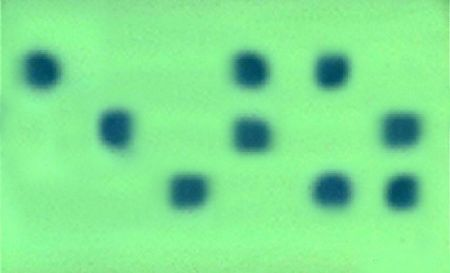
\includegraphics[width=1\textwidth]{images_20170905_allozymes.jpg}
     	\end{center}
		\end{column}
	\end{columns}
\end{frame}

%------------------------------------------------
\begin{frame}
\frametitle{Sanger Sequencing}
\begin{itemize}
	\item 1977
	\item Determines the sequences a single piece of DNA up to 500bp
	\item Highly accurate but slow
\end{itemize}
\end{frame}

%------------------------------------------------
\begin{frame}
\frametitle{Sanger Sequencing}
\begin{columns}
	\begin{column}{0.5\textwidth}
		\begin{itemize}
			\item Design a primer
			\item Run a PCR
			\item Chain-terminating dideoxynucleotide triphosphates
		\end{itemize}
	\end{column}
	\begin{column}{0.5\textwidth}
    	\begin{center}
     		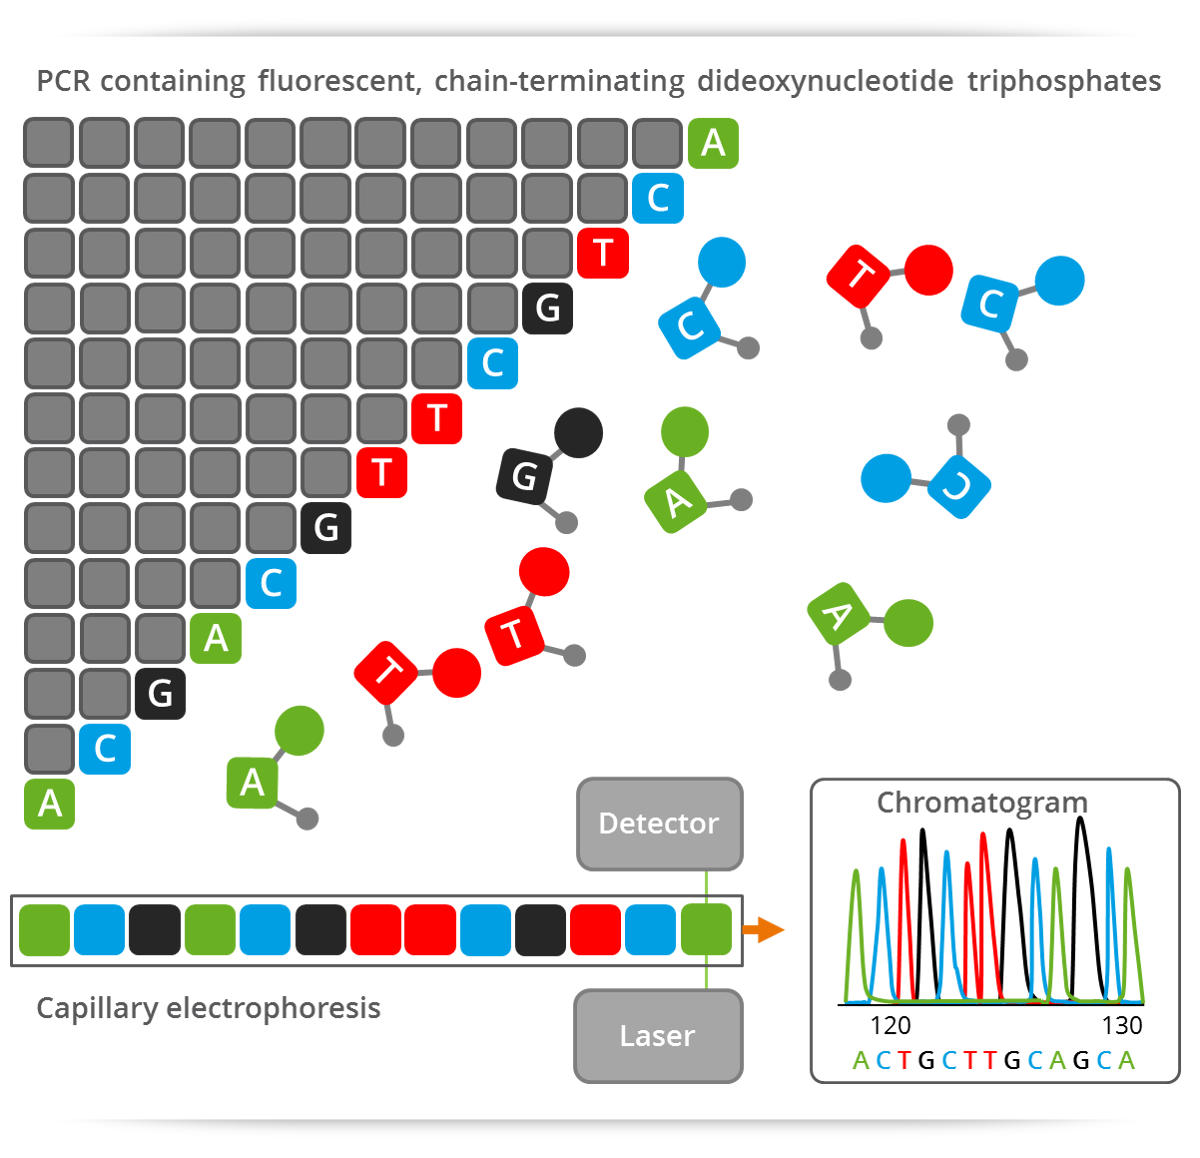
\includegraphics[width=1\textwidth]{images_20170905_sanger.jpg}
     	\end{center}
		\end{column}
	\end{columns}
\end{frame}

%------------------------------------------------
\begin{frame}
\frametitle{Sanger Sequencing}
\begin{columns}
	\begin{column}{0.5\textwidth}
		\begin{itemize}
			\item Run results on a gel
			\item Read with a laser, determines which base ended the PCR
			\item Color order is sequence order
		\end{itemize}
	\end{column}
	\begin{column}{0.5\textwidth}
    	\begin{center}
     		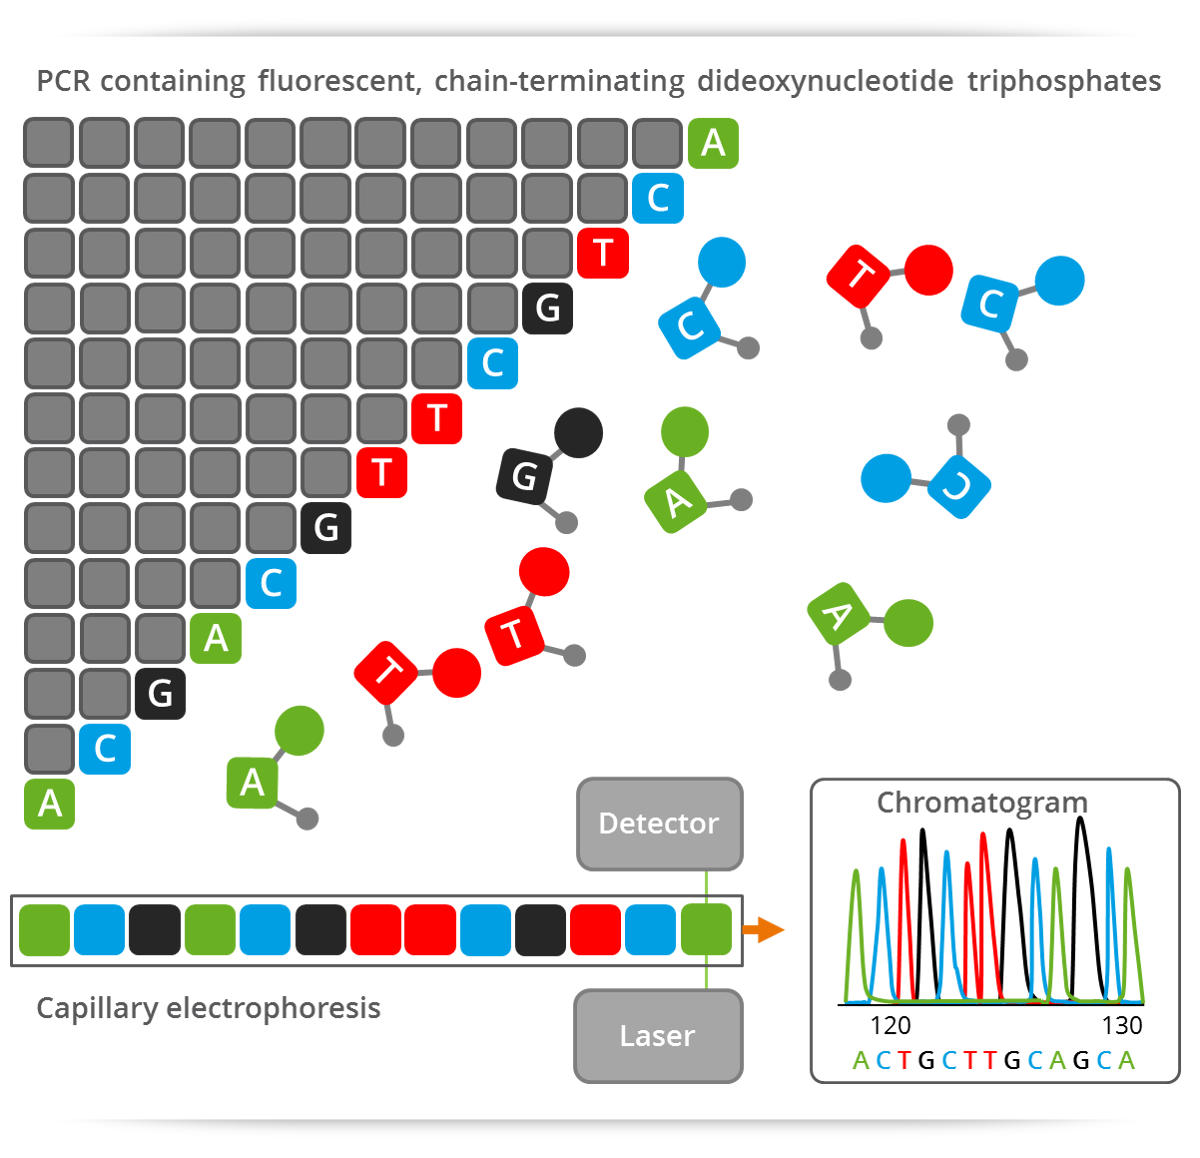
\includegraphics[width=1\textwidth]{images_20170905_sanger.jpg}
     	\end{center}
		\end{column}
	\end{columns}
\end{frame}

%------------------------------------------------
\begin{frame}
\frametitle{NGS Sequencing}
\begin{itemize}
	\item mid-2000's
	\item Many different companies and methods
	\item All generate far more data than Sanger
\end{itemize}
\end{frame}

%------------------------------------------------
\begin{frame}
\frametitle{NGS Sequencing - Illumina}
\begin{columns}
	\begin{column}{0.5\textwidth}
		\begin{itemize}
			\item Library Preparation
			\begin{itemize}
				\item Fragment a sample of whole genomic DNA
				\item Add adapters for the specific machine
			\end{itemize}
			\item Amplify with PCR
			\item Read on machine (next slide)
		\end{itemize}
	\end{column}
	\begin{column}{0.5\textwidth}
    	\begin{center}
     		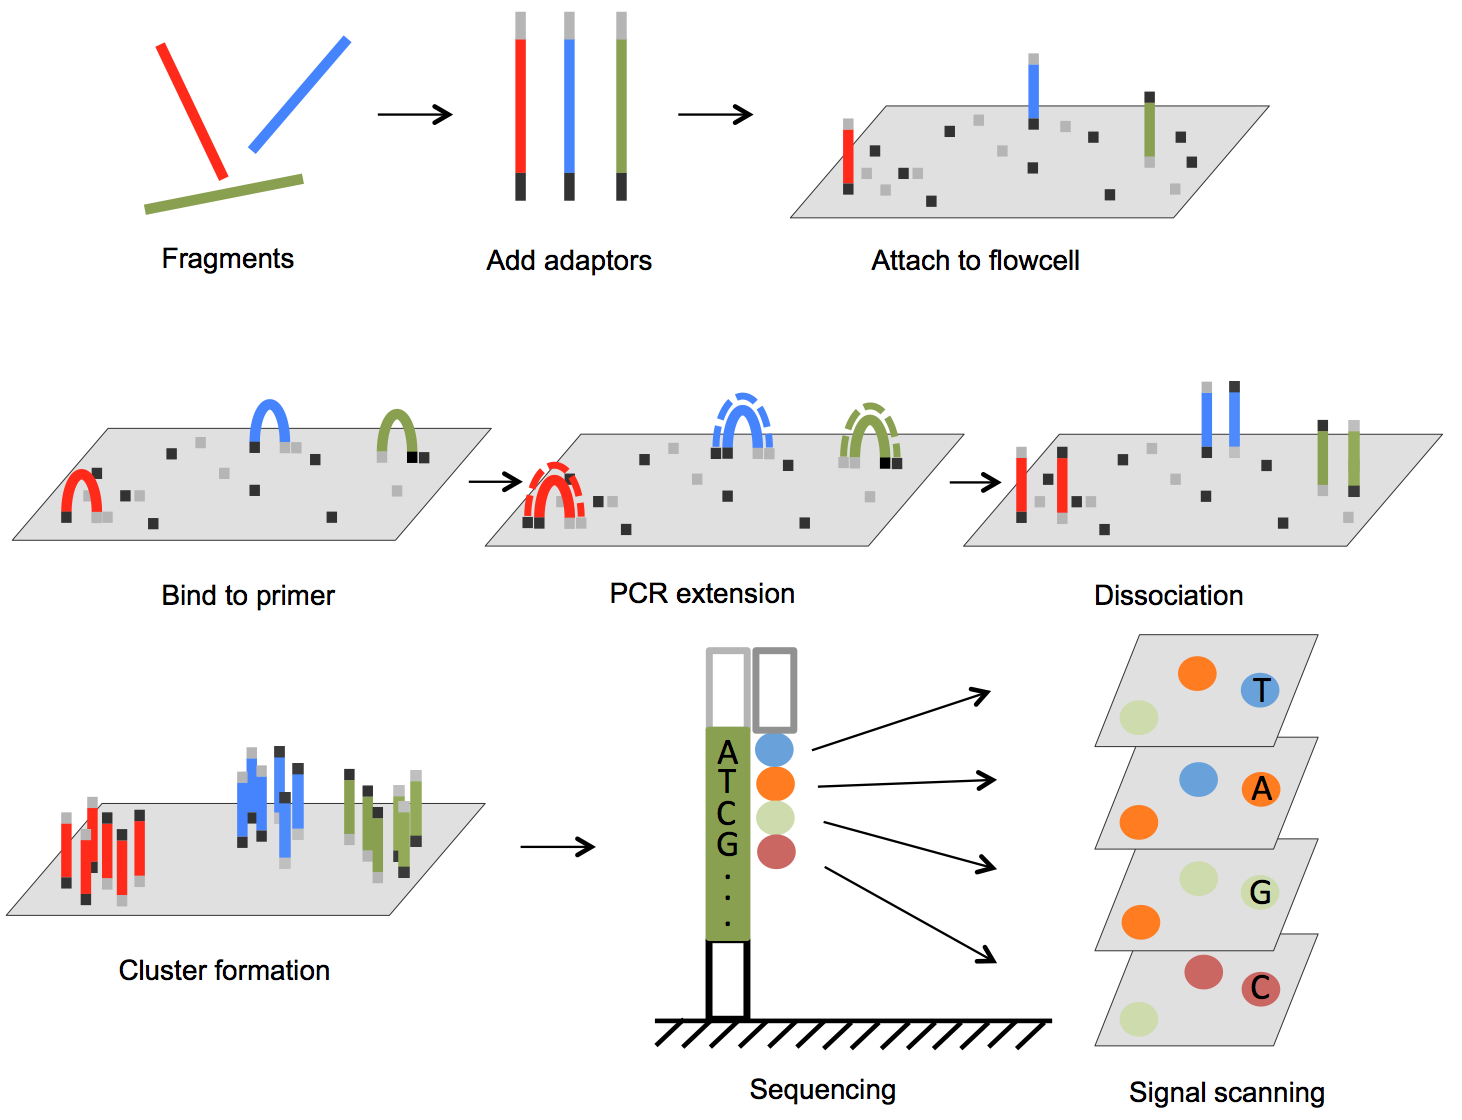
\includegraphics[width=1\textwidth]{images_20170905_illumina.png}
     	\end{center}
		\end{column}
	\end{columns}
\end{frame}

%------------------------------------------------
\begin{frame}
\frametitle{NGS Sequencing - Illumina}
\begin{columns}
	\begin{column}{0.5\textwidth}
		\begin{itemize}
			\item Machine attaches adapter and DNA to a fixed surface
			\item Amplifies single strand
			\item Adds a new base each cycle and images for ID
		\end{itemize}
	\end{column}
	\begin{column}{0.5\textwidth}
    	\begin{center}
     		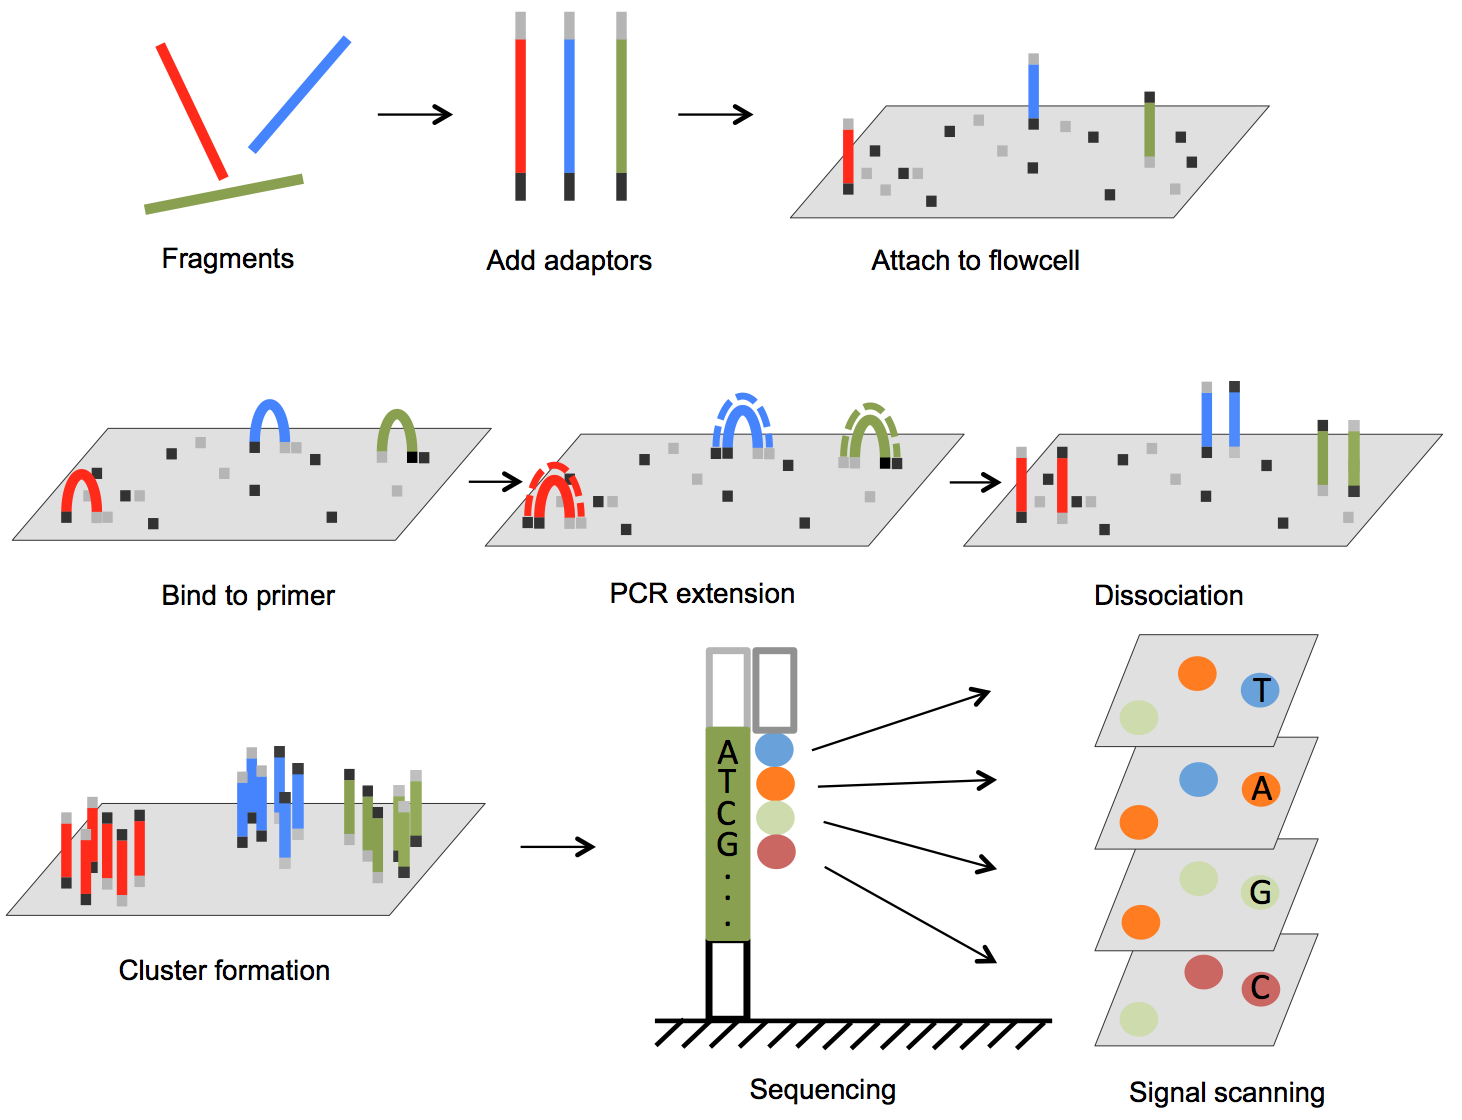
\includegraphics[width=1\textwidth]{images_20170905_illumina.png}
     	\end{center}
		\end{column}
	\end{columns}
\end{frame}

%------------------------------------------------
\begin{frame}
\frametitle{NGS Sequencing - PacBio}
\begin{columns}
	\begin{column}{0.5\textwidth}
		\begin{itemize}
			\item Library Preparation
			\begin{itemize}
				\item Fragment a sample of whole genomic DNA
				\item Add adapters for the specific machine
			\end{itemize}
			\item Amplify with PCR
			\item Read on machine
		\end{itemize}
	\end{column}
	\begin{column}{0.5\textwidth}
    	\begin{center}
     		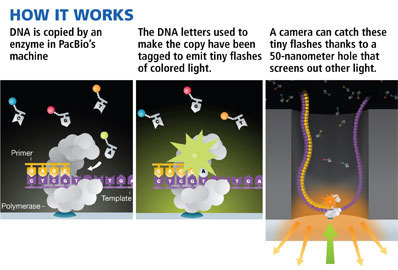
\includegraphics[width=1\textwidth]{images_20170905_pacbio.jpg}
     	\end{center}
		\end{column}
	\end{columns}
\end{frame}

%------------------------------------------------
\begin{frame}
\frametitle{NGS Sequencing - PacBio}
\begin{columns}
	\begin{column}{0.5\textwidth}
		\begin{itemize}
			\item A copy is made on the machine by an enzyme
			\item The bases used for the copy are flourescent
			\item As a new base is incorporated the color shows the identity
		\end{itemize}
	\end{column}
	\begin{column}{0.5\textwidth}
    	\begin{center}
     		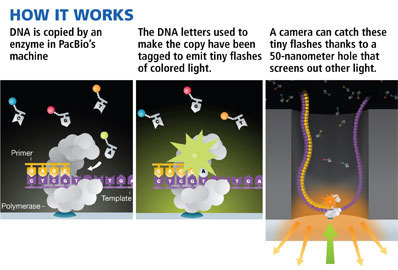
\includegraphics[width=1\textwidth]{images_20170905_pacbio.jpg}
     	\end{center}
		\end{column}
	\end{columns}
\end{frame}

%------------------------------------------------
\begin{frame}
\frametitle{Next Generation Sequencing vs. Sanger}
\begin{itemize}
	\item<1-> Output for Quality Tradeoff
	\begin{itemize}
		\item NGS = VERY High Output / Good Quality
		\item Sanger = Low Output / Best Quality
	\end{itemize}
	\item<2-> NGS Methods and Machines
	\begin{itemize}
		\item<3-> PyroSeq - 454
		\item<4-> Illumina
		\item<5-> PacBio
	\end{itemize}
\end{itemize}
\end{frame}

%------------------------------------------------
\begin{frame}
\frametitle{Brief History of Sequencing}
\begin{itemize}
	\item Allozymes
	\begin{itemize}
		\item 1960's
	\end{itemize}
	\item Sanger Sequencing
	\begin{itemize}
		\item 1977
	\end{itemize}
	\item NGS - Next Generation Sequencing
	\begin{itemize}
		\item 2000
	\end{itemize}
\end{itemize}
\end{frame}

%------------------------------------------------
\begin{frame}
\begin{figure}

\includegraphics[width=0.8\linewidth]{images_20170829_NGS_meme.png}
\end{figure}
\end{frame}

%------------------------------------------------
\begin{frame}
\frametitle{Sequencing Cost}
\begin{figure}
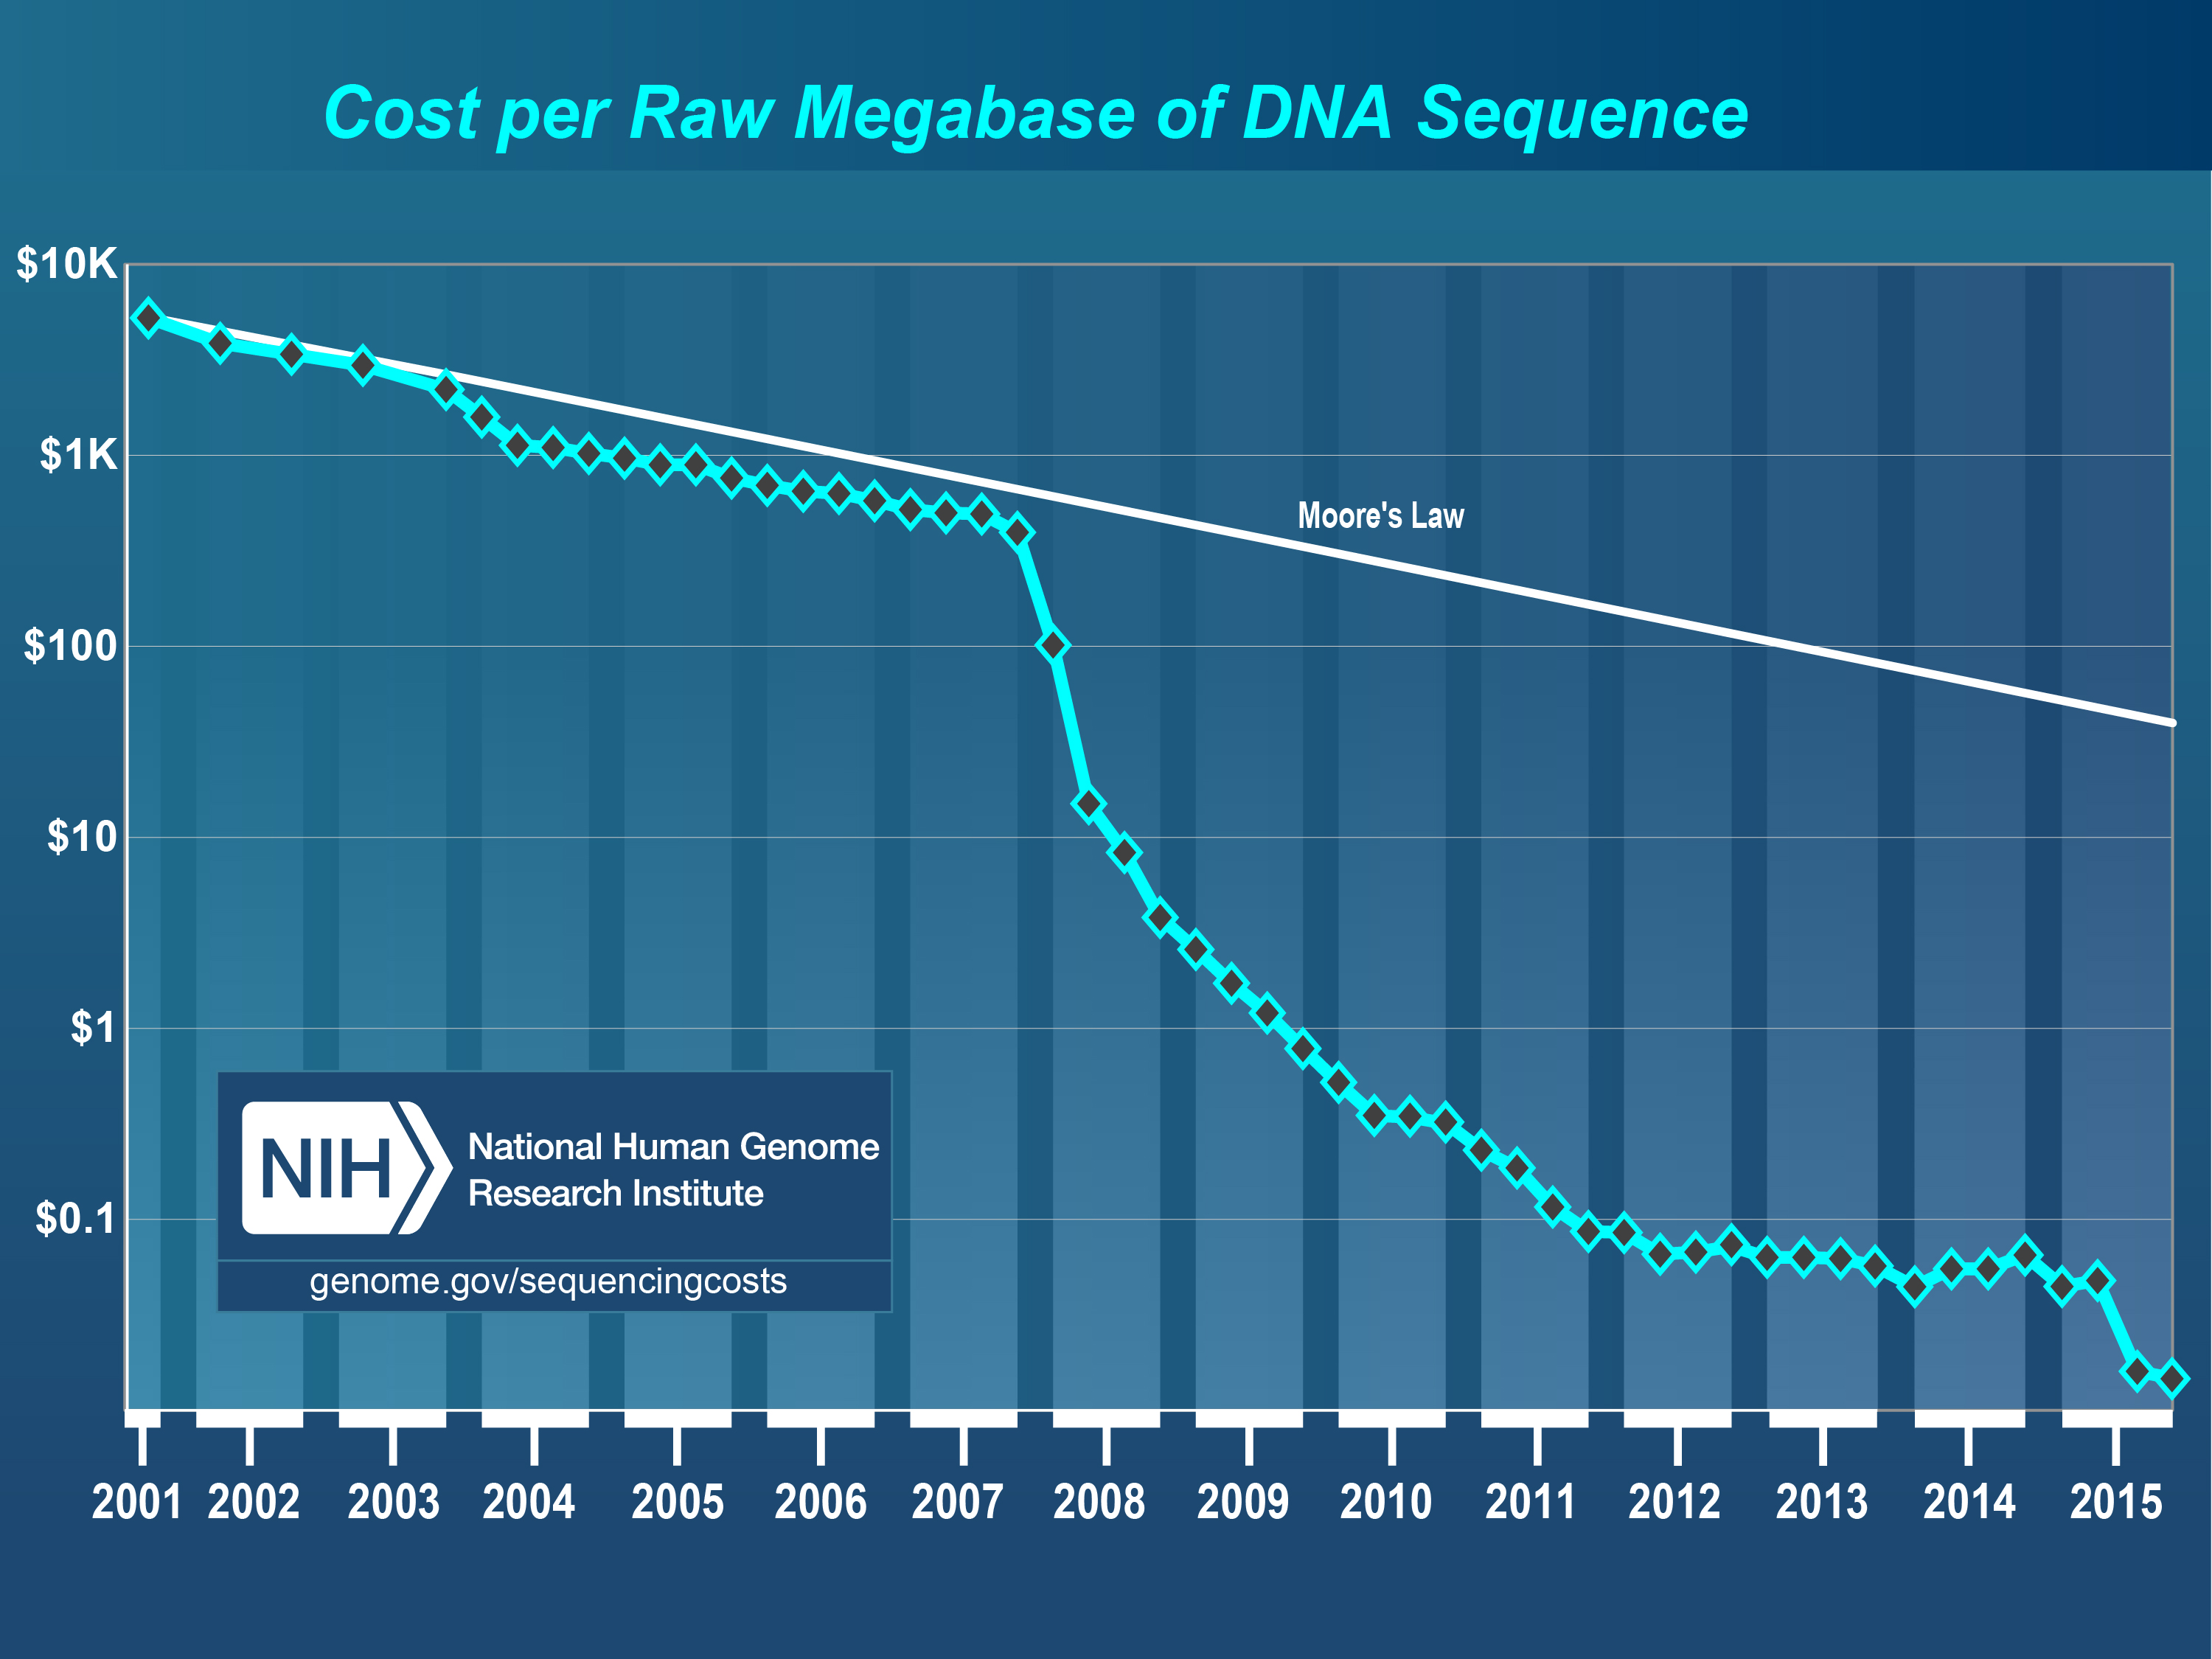
\includegraphics[width=0.8\linewidth]{images_20170829_NGS_cost.jpg}
\end{figure}
\end{frame}

%------------------------------------------------
\begin{frame}
\frametitle{Sequencing Output}
\begin{figure}
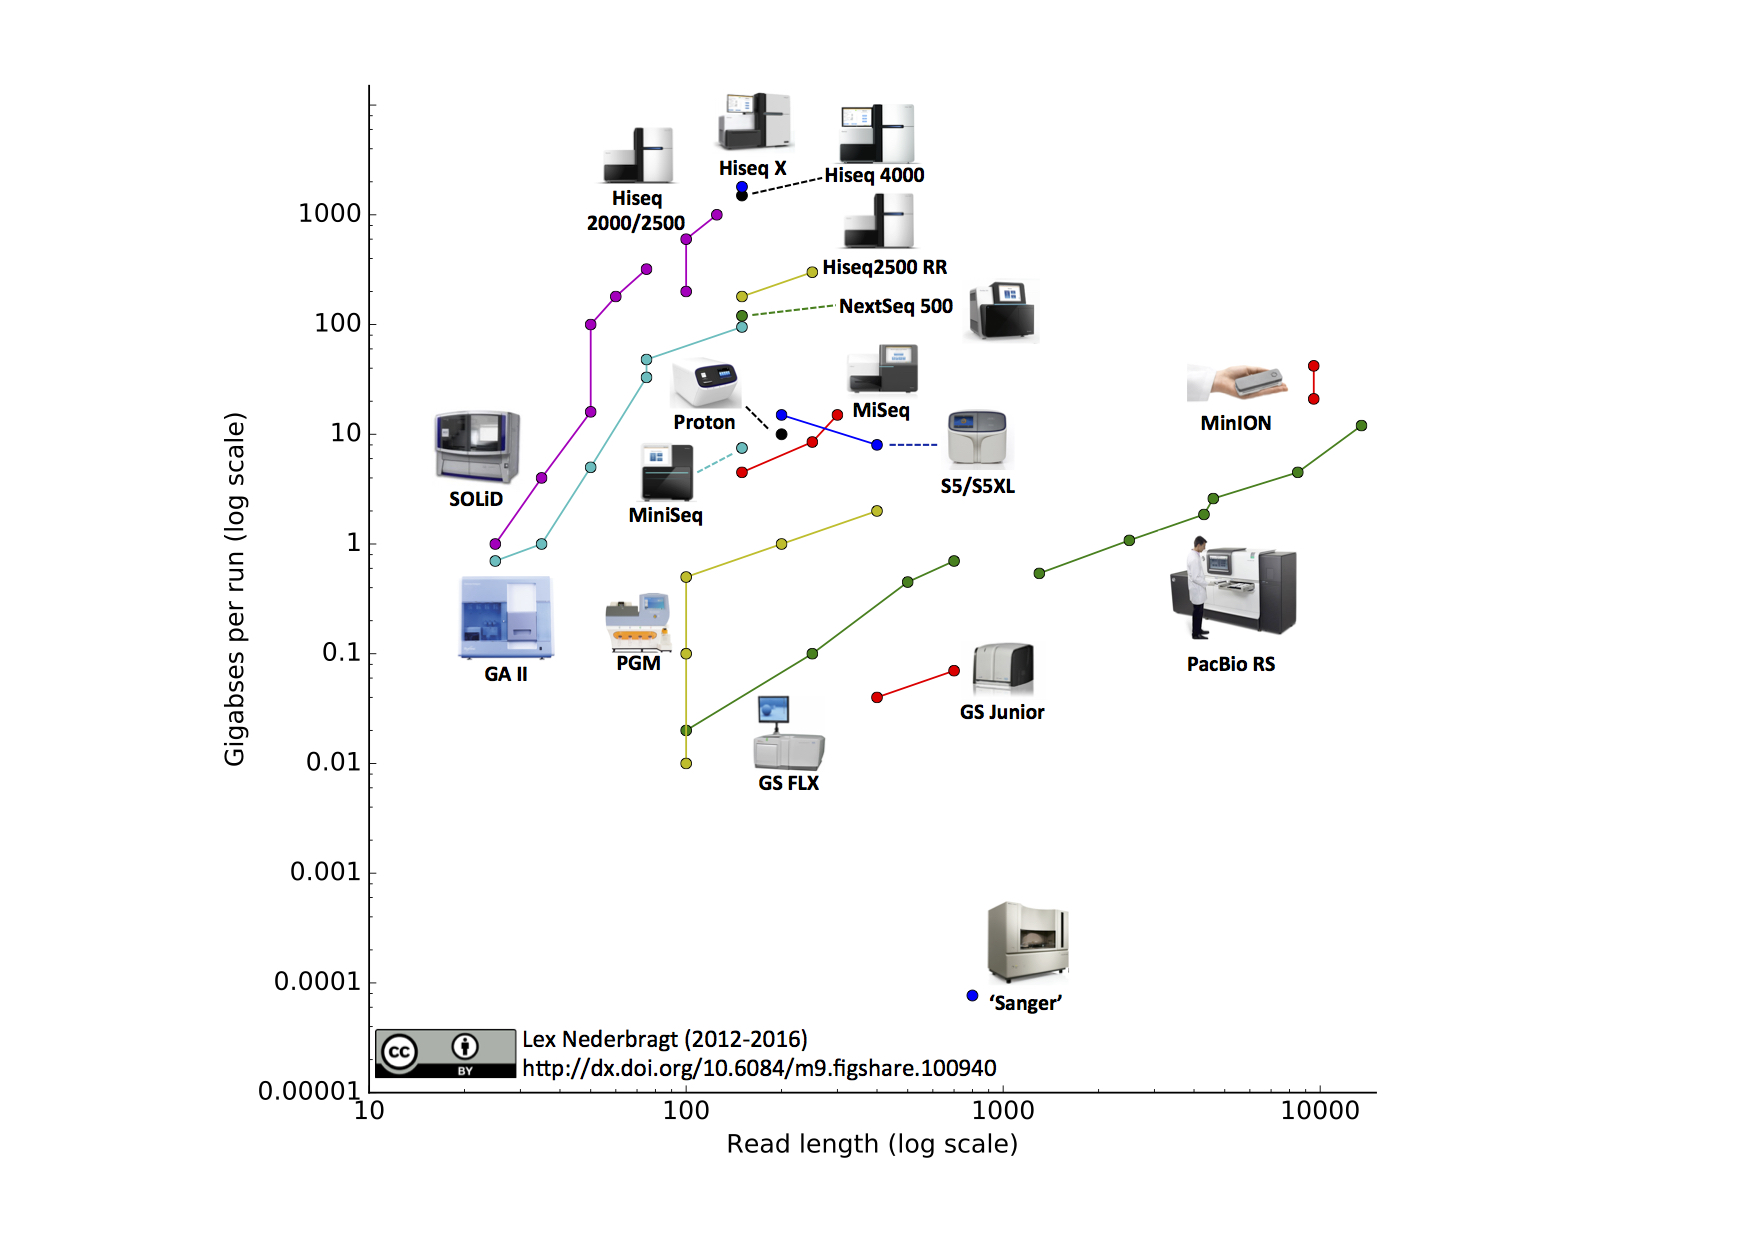
\includegraphics[width=0.8\linewidth]{images_20170829_machine_output.jpg}
\end{figure}
\end{frame}

%------------------------------------------------
\begin{frame}
\frametitle{Generational Shift}
\begin{itemize}
	\item<1-> More and more data can be generated
	\item<2-> Data length and quality are both improving
	\item<3-> How does this change the scope of research?
\end{itemize}
\end{frame}

%------------------------------------------------
\section{In-Class Activity}

%------------------------------------------------
\begin{frame}
\frametitle{In-Class Activity}
	\begin{enumerate}
	\item<1-> Make 4 groups (rearrange desks)
	\item<2-> Divide up the following Biological Questions
		\begin{itemize}
			\item<3-> How similar are two species?
			\item<4-> What genes underlie a specific function?
			\item<5-> What is the code of the human genome?
			\item<6-> Group's Choice:
			\begin{itemize}
			\item Transcription Factors
			\item CpG islands
			\item DNA Methylation
			\end{itemize}
		\end{itemize}
	\item<7-> How would your group assess this question 
	\begin{itemize}
		\item in 1997?
		\item in 2017?
	\end{itemize}
	\end{enumerate}
\end{frame}
%%%%%%%%%%%%%%%%%%%%%%%%%%%%%%%%%%%%%%%%%%%%%%%%%%%%%%%%%%%%
%% REMOVE COMMENTS HERE AND RE-BUILD LOCALLY BEFORE CLASS %%
%%%%%%%%%%%%%%%%%%%%%%%%%%%%%%%%%%%%%%%%%%%%%%%%%%%%%%%%%%%%
%%                  AND DON'T COMMIT                      %%
%%%%%%%%%%%%%%%%%%%%%%%%%%%%%%%%%%%%%%%%%%%%%%%%%%%%%%%%%%%%
%------------------------------------------------
\begin{frame}
	\begin{itemize}
		\item<+-> {\Large Group Choice Order:}
		\item<+-> Close your laptops/phones
		\item<+-> In your group take 60 seconds to answer the following:
		\item<+-> How many basepairs are in the human genome?
		\item<+-> ---------
		\item<+-> 3,234.83 Mb
	\end{itemize}
\end{frame}

\begin{frame}
\frametitle{Function}
	\begin{itemize}
		\item 2017
		\item easily ask question bc you can completely sequence the genome
		\item RNAseq 
		\item knockout screen - knock sections out and see changes
		\item 1997
		\item asl the question in a limited way - how does a single gene alter a single function
	\end{itemize}
\end{frame}

\begin{frame}
\frametitle{Transcription Factor}
	\begin{itemize}
		\item Transcription Factor - protien that regulates the transcription of a gene
		\item feedback loops in gene pathways
		\item 1997
		\item knockouts and broad genetic methods
		\item ask about a known TF
		\item 2017
		\item CHIPseq - chromatin immunoprecipitation seq
		\item digest DNA, protect areas that are bound to protein
		\item assess which TFs are present
		\item correlative but guides future research
	\end{itemize}
\end{frame}

\begin{frame}
\frametitle{Genome Assembly}
	\begin{itemize}
		\item 1997
		\item broke down the genome into 150k bp frags
		\item cloned fragments
		\item broke down again
		\item cloned and Sanger sequenced
		\item 2017
		\item easy to get a lot of data
		\item hard to assess repetitive regions
		\item combine illumina and pacbio data
	\end{itemize}
\end{frame}


\begin{frame}
\frametitle{PopGen}
	\begin{itemize}
		\item 1997
		\item sanger sequence conserved genes
		\item 2017
		\item whole genome seq
		\item RADseq - focus on shared areas across species
	\end{itemize}
\end{frame}

%------------------------------------------------
\begin{frame}
\Huge{\centerline{The End}}
\end{frame}

%----------------------------------------------------------------------------------------

\end{document} 